\section{Etude de l'impact de l'arrêt de la PDSA}

Regarder d'une part 1) l'activité pour chaque SU, avec pour le total des
passages aux SU - le nombre de CCMU 1 - le nombre de CCMU2 - en fonction
des périodes horaires indiquées ci-dessous

En regardant l'évolution du chiffre par semaine, et par mois: une
représentation par graphique pourrait être intéressante si cela est
possible. Cette première étape vise à observer l'évolution du nombre de
CCMU1 sur l'ensemble de l'année, par période horaire (avant/après
minuit), sur le nombre total de passage aux urgence: par exemple, en
figurant sur un premier graphique: une courbe des CCMU1 avant minuit
avec une courbe du nombre de passage total aux SU, et sur un 2e
graphique: une courbe des CCMU1 après minuit avec une courbe du nombre
de passage total aux SU.

et d'autre part

\begin{enumerate}
\def\labelenumi{\arabic{enumi})}
\setcounter{enumi}{1}
\itemsep1pt\parskip0pt\parsep0pt
\item
  en croisant le nombre de CCMU1 selon la tranche horaire (avant
  minuit/après minuit) en fonction des territoires de PDSA dont viennent
  les patients (en utilisant le code postal des patients pour recoder la
  porvenance du territoire): la question étant= sur toutes les CCMU1
  observées après minuit dans chaque SU, il y a-t-il significativement
  plus de patients en provenance des territoires où la PDSA s'est
  arrêtée? Cette deuxième étape viserait à identifier plus finement si
  une éventuelle augmentation de CCMU1 peut être attribuée à la
  provenance des patients (territoire de PDSA).
\end{enumerate}

L'autre fichier Excel fournit hier permettra d'interpréter les données
en fonction des dates d'arrêt de PDSA après minuit dans certains
territoires.

\subsection{Initialisation}

dim. 09 févr. 2014 (10:59:27)

On crée deux groupes: - soirée (SR) dsr - nuit profonde (NP) dnp

\begin{Shaded}
\begin{Highlighting}[]
\KeywordTok{library}\NormalTok{(}\StringTok{"lubridate"}\NormalTok{, }\DataTypeTok{lib.loc =} \StringTok{"/home/jcb/R/x86_64-pc-linux-gnu-library/3.0"}\NormalTok{)}
\KeywordTok{library}\NormalTok{(}\StringTok{"epicalc"}\NormalTok{, }\DataTypeTok{lib.loc =} \StringTok{"/usr/lib/R/site-library"}\NormalTok{)}
\end{Highlighting}
\end{Shaded}

\begin{verbatim}
## Loading required package: foreign
## Loading required package: survival
## Loading required package: splines
## Loading required package: MASS
## Loading required package: nnet
\end{verbatim}

\begin{Shaded}
\begin{Highlighting}[]
\KeywordTok{load}\NormalTok{(}\StringTok{"~/Documents/Resural/Stat Resural/RPU_2013/rpu2013d0112.Rda"}\NormalTok{)}
\NormalTok{dx <-}\StringTok{ }\NormalTok{d1[, }\KeywordTok{c}\NormalTok{(}\StringTok{"ENTREE"}\NormalTok{, }\StringTok{"FINESS"}\NormalTok{, }\StringTok{"GRAVITE"}\NormalTok{)]}
\CommentTok{# groupe soirée}
\NormalTok{dsr <-}\StringTok{ }\NormalTok{dx[}\KeywordTok{hour}\NormalTok{(dx$ENTREE) >}\StringTok{ }\DecValTok{19} \NormalTok{&}\StringTok{ }\KeywordTok{hour}\NormalTok{(dx$ENTREE) <}\StringTok{ }\DecValTok{24}\NormalTok{, ]}
\NormalTok{dsr$GRP <-}\StringTok{ "SR"}
\CommentTok{# groupe nuit profonde}
\NormalTok{dnp <-}\StringTok{ }\NormalTok{dx[}\KeywordTok{hour}\NormalTok{(dx$ENTREE) >=}\StringTok{ }\DecValTok{0} \NormalTok{&}\StringTok{ }\KeywordTok{hour}\NormalTok{(dx$ENTREE) <}\StringTok{ }\DecValTok{8}\NormalTok{, ]}
\NormalTok{dnp$GRP <-}\StringTok{ "NP"}
\CommentTok{# synthèse des deux}
\NormalTok{dx2 <-}\StringTok{ }\KeywordTok{rbind}\NormalTok{(dsr, dnp)}
\end{Highlighting}
\end{Shaded}

\subsection{Nombre total de passages}

\begin{Shaded}
\begin{Highlighting}[]
\NormalTok{n_tot <-}\StringTok{ }\KeywordTok{nrow}\NormalTok{(d1)}
\NormalTok{n_soirnuit <-}\StringTok{ }\KeywordTok{nrow}\NormalTok{(dx2)}
\end{Highlighting}
\end{Shaded}

\begin{itemize}
\itemsep1pt\parskip0pt\parsep0pt
\item
  total des passages en 2013: 340338
\item
  entre 20h et 8h: 96874 (28.46 \%)
\item
  dont
\item
  soirée (20h-0h): 59475 (17.48 \%)
\item
  nuit profonde (0h-8h): 37399 (10.99 \%)
\end{itemize}

\subsection{Analyse CCMU}

\begin{Shaded}
\begin{Highlighting}[]
\KeywordTok{tab1}\NormalTok{(dx$GRAVITE, }\DataTypeTok{main =} \StringTok{"2013 - Gravité (en unités CCMU)"}\NormalTok{, }\DataTypeTok{ylab =} \StringTok{"Fréquence"}\NormalTok{, }
    \DataTypeTok{xlab =} \StringTok{"CCMU"}\NormalTok{)}
\end{Highlighting}
\end{Shaded}

\begin{figure}[htbp]
\centering
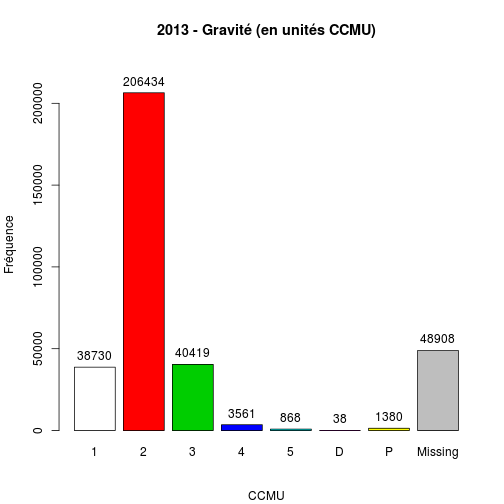
\includegraphics{figure/ccmu1.png}
\caption{plot of chunk ccmu}
\end{figure}

\begin{verbatim}
## dx$GRAVITE : 
##         Frequency   %(NA+)   %(NA-)
## 1           38730     11.4     13.3
## 2          206434     60.7     70.8
## 3           40419     11.9     13.9
## 4            3561      1.0      1.2
## 5             868      0.3      0.3
## D              38      0.0      0.0
## P            1380      0.4      0.5
## NA's        48908     14.4      0.0
##   Total    340338    100.0    100.0
\end{verbatim}

\begin{Shaded}
\begin{Highlighting}[]

\KeywordTok{tab1}\NormalTok{(dsr$GRAVITE, }\DataTypeTok{main =} \StringTok{"2013 - Groupe soirée (20h - minuit)"}\NormalTok{)}
\end{Highlighting}
\end{Shaded}

\begin{figure}[htbp]
\centering
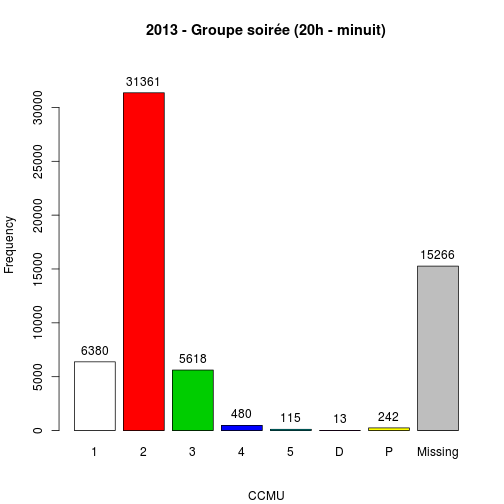
\includegraphics{figure/ccmu2.png}
\caption{plot of chunk ccmu}
\end{figure}

\begin{verbatim}
## dsr$GRAVITE : 
##         Frequency   %(NA+)   %(NA-)
## 1            6380     10.7     14.4
## 2           31361     52.7     70.9
## 3            5618      9.4     12.7
## 4             480      0.8      1.1
## 5             115      0.2      0.3
## D              13      0.0      0.0
## P             242      0.4      0.5
## NA's        15266     25.7      0.0
##   Total     59475    100.0    100.0
\end{verbatim}

\begin{Shaded}
\begin{Highlighting}[]

\KeywordTok{tab1}\NormalTok{(dnp$GRAVITE, }\DataTypeTok{main =} \StringTok{"2013 - Groupe nuit profonde (0h - 8h)"}\NormalTok{)}
\end{Highlighting}
\end{Shaded}

\begin{figure}[htbp]
\centering
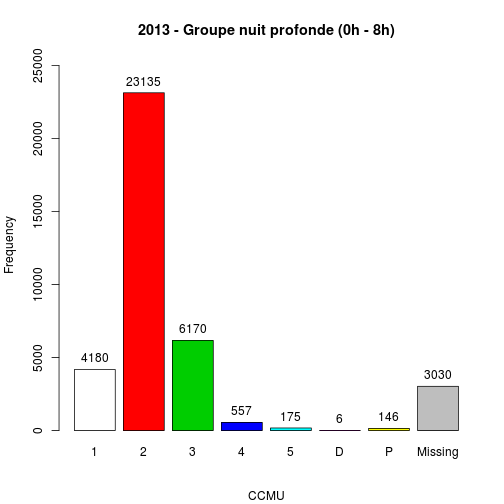
\includegraphics{figure/ccmu3.png}
\caption{plot of chunk ccmu}
\end{figure}

\begin{verbatim}
## dnp$GRAVITE : 
##         Frequency   %(NA+)   %(NA-)
## 1            4180     11.2     12.2
## 2           23135     61.9     67.3
## 3            6170     16.5     18.0
## 4             557      1.5      1.6
## 5             175      0.5      0.5
## D               6      0.0      0.0
## P             146      0.4      0.4
## NA's         3030      8.1      0.0
##   Total     37399    100.0    100.0
\end{verbatim}

\begin{Shaded}
\begin{Highlighting}[]

\NormalTok{t <-}\StringTok{ }\KeywordTok{table}\NormalTok{(dx2$GRP, dx2$GRAVITE)}
\NormalTok{t}
\end{Highlighting}
\end{Shaded}

\begin{verbatim}
##     
##          1     2     3     4     5     D     P
##   NP  4180 23135  6170   557   175     6   146
##   SR  6380 31361  5618   480   115    13   242
\end{verbatim}

\begin{Shaded}
\begin{Highlighting}[]
\CommentTok{# on permute les lignes pour que SR précède NP}
\NormalTok{a <-}\StringTok{ }\NormalTok{t[}\DecValTok{1}\NormalTok{, ]}
\NormalTok{b <-}\StringTok{ }\NormalTok{t[}\DecValTok{2}\NormalTok{, ]}
\NormalTok{t <-}\StringTok{ }\KeywordTok{rbind}\NormalTok{(b, a)}
\KeywordTok{rownames}\NormalTok{(t) <-}\StringTok{ }\KeywordTok{c}\NormalTok{(}\StringTok{"SR"}\NormalTok{, }\StringTok{"NP"}\NormalTok{)}
\NormalTok{pt <-}\StringTok{ }\KeywordTok{round}\NormalTok{(}\KeywordTok{prop.table}\NormalTok{(t, }\DataTypeTok{margin =} \DecValTok{1}\NormalTok{) *}\StringTok{ }\DecValTok{100}\NormalTok{, }\DecValTok{2}\NormalTok{)}
\NormalTok{t}
\end{Highlighting}
\end{Shaded}

\begin{verbatim}
##       1     2    3   4   5  D   P
## SR 6380 31361 5618 480 115 13 242
## NP 4180 23135 6170 557 175  6 146
\end{verbatim}

\begin{Shaded}
\begin{Highlighting}[]
\NormalTok{pt}
\end{Highlighting}
\end{Shaded}

\begin{verbatim}
##        1     2     3    4    5    D    P
## SR 14.43 70.94 12.71 1.09 0.26 0.03 0.55
## NP 12.16 67.31 17.95 1.62 0.51 0.02 0.42
\end{verbatim}

\begin{Shaded}
\begin{Highlighting}[]
\KeywordTok{barplot}\NormalTok{(pt, }\DataTypeTok{beside =} \OtherTok{TRUE}\NormalTok{, }\DataTypeTok{ylab =} \StringTok{"pourcentage"}\NormalTok{, }\DataTypeTok{xlab =} \StringTok{"CCMU en soirée et nuit profonde"}\NormalTok{, }
    \DataTypeTok{main =} \StringTok{"Comparaison des CCMU avant et après minuit"}\NormalTok{)}
\KeywordTok{legend}\NormalTok{(}\StringTok{"topright"}\NormalTok{, }\DataTypeTok{legend =} \KeywordTok{c}\NormalTok{(}\StringTok{"0h-24h"}\NormalTok{, }\StringTok{"24h-8h"}\NormalTok{), }\DataTypeTok{pch =} \DecValTok{15}\NormalTok{, }\DataTypeTok{col =} \KeywordTok{c}\NormalTok{(}\StringTok{"grey10"}\NormalTok{, }
    \StringTok{"grey90"}\NormalTok{))}
\end{Highlighting}
\end{Shaded}

\begin{figure}[htbp]
\centering
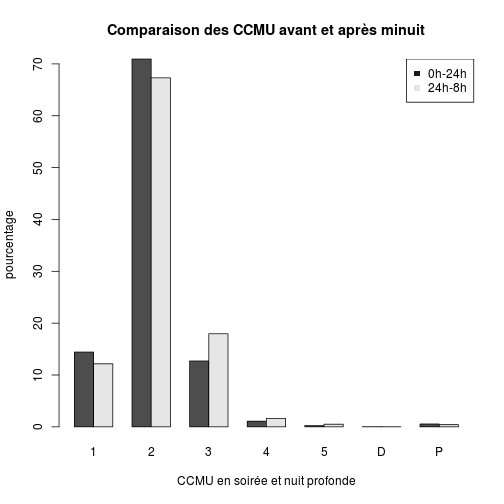
\includegraphics{figure/ccmu4.png}
\caption{plot of chunk ccmu}
\end{figure}

\subsection{Analyse des CCMU1 \& 2 par mois et semaine}

\begin{itemize}
\item
  dsr1: soirée, ccmu1
\item
  dsr2: soirée, ccmu2
\item
  dsrt: soirée, total (sans les NA)
\item
  t\_dsr1: soirée, ccmu1 par mois
\item
  t\_dsr2: soirée, ccmu2 par mois
\item
  t\_dsrt
\item
  dnp1: nuit profonde, ccmu1
\item
  dnp2: nuit profonde, ccmu2
\item
  dnpt: nuit profonde, total (sans les NA)
\item
  t\_dnp1: nuit profonde, ccmu1 par mois
\item
  t\_dnp2: nuit profonde, ccmu2 par mois
\item
  t\_dnpt: nuit profonde, total par mois
\end{itemize}

\begin{Shaded}
\begin{Highlighting}[]

\CommentTok{# soirée ----------}
\NormalTok{dsr1 <-}\StringTok{ }\NormalTok{dsr[!}\KeywordTok{is.na}\NormalTok{(dsr$GRAVITE) &}\StringTok{ }\NormalTok{dsr$GRAVITE ==}\StringTok{ }\DecValTok{1}\NormalTok{, ]}
\NormalTok{dsr2 <-}\StringTok{ }\NormalTok{dsr[!}\KeywordTok{is.na}\NormalTok{(dsr$GRAVITE) &}\StringTok{ }\NormalTok{dsr$GRAVITE ==}\StringTok{ }\DecValTok{2}\NormalTok{, ]}
\NormalTok{dsrt <-}\StringTok{ }\NormalTok{dsr[!}\KeywordTok{is.na}\NormalTok{(dsr$GRAVITE), ]}

\NormalTok{t_dsr1 <-}\StringTok{ }\KeywordTok{tapply}\NormalTok{(dsr1$GRAVITE, }\KeywordTok{month}\NormalTok{(}\KeywordTok{as.Date}\NormalTok{(dsr1$ENTREE)), length)}
\NormalTok{t_dsr2 <-}\StringTok{ }\KeywordTok{tapply}\NormalTok{(dsr2$GRAVITE, }\KeywordTok{month}\NormalTok{(}\KeywordTok{as.Date}\NormalTok{(dsr2$ENTREE)), length)}
\NormalTok{t_dsrt <-}\StringTok{ }\KeywordTok{tapply}\NormalTok{(dsr$GRAVITE, }\KeywordTok{month}\NormalTok{(}\KeywordTok{as.Date}\NormalTok{(dsr$ENTREE)), length)}
\NormalTok{sr <-}\StringTok{ }\KeywordTok{rbind}\NormalTok{(t_dsr1, t_dsr2, t_dsrt)}
\KeywordTok{barplot}\NormalTok{(sr, }\DataTypeTok{beside =} \NormalTok{T, }\DataTypeTok{ylab =} \StringTok{"Freéquence"}\NormalTok{, }\DataTypeTok{xlab =} \StringTok{"Mois"}\NormalTok{, }\DataTypeTok{main =} \StringTok{"CCMU 2013 - Soirée"}\NormalTok{)}
\KeywordTok{legend}\NormalTok{(}\StringTok{"topleft"}\NormalTok{, }\DataTypeTok{legend =} \KeywordTok{c}\NormalTok{(}\StringTok{"CCMU 1"}\NormalTok{, }\StringTok{"CCMU 2"}\NormalTok{, }\StringTok{"Total RPU"}\NormalTok{), }\DataTypeTok{col =} \KeywordTok{c}\NormalTok{(}\StringTok{"gray10"}\NormalTok{, }
    \StringTok{"gray50"}\NormalTok{, }\StringTok{"gray90"}\NormalTok{), }\DataTypeTok{pch =} \DecValTok{15}\NormalTok{, }\DataTypeTok{bty =} \StringTok{"n"}\NormalTok{)}
\end{Highlighting}
\end{Shaded}

\begin{figure}[htbp]
\centering
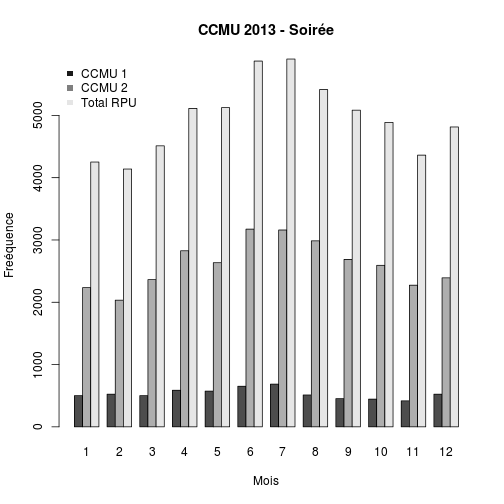
\includegraphics{figure/mois1.png}
\caption{plot of chunk mois}
\end{figure}

\begin{Shaded}
\begin{Highlighting}[]

\KeywordTok{plot}\NormalTok{(t_dsr1, }\DataTypeTok{type =} \StringTok{"l"}\NormalTok{, }\DataTypeTok{ylim =} \KeywordTok{c}\NormalTok{(}\DecValTok{450}\NormalTok{, }\DecValTok{3500}\NormalTok{), }\DataTypeTok{col =} \StringTok{"green"}\NormalTok{)}
\KeywordTok{lines}\NormalTok{(t_dsr2, }\DataTypeTok{ylim =} \KeywordTok{c}\NormalTok{(}\DecValTok{450}\NormalTok{, }\DecValTok{3500}\NormalTok{), }\DataTypeTok{col =} \StringTok{"blue"}\NormalTok{)}
\end{Highlighting}
\end{Shaded}

\begin{figure}[htbp]
\centering
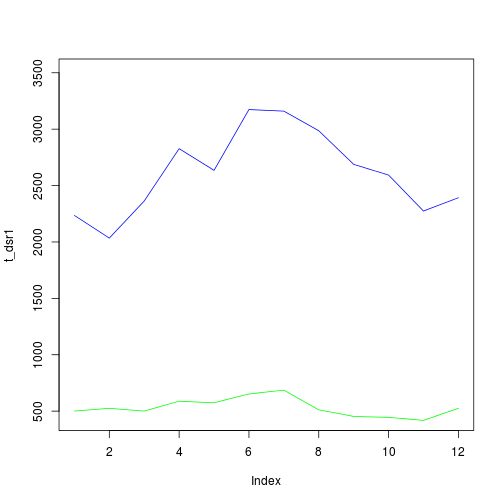
\includegraphics{figure/mois2.png}
\caption{plot of chunk mois}
\end{figure}

\begin{Shaded}
\begin{Highlighting}[]

\CommentTok{# nuit profonde --------------}

\NormalTok{dnp1 <-}\StringTok{ }\NormalTok{dnp[!}\KeywordTok{is.na}\NormalTok{(dnp$GRAVITE) &}\StringTok{ }\NormalTok{dnp$GRAVITE ==}\StringTok{ }\DecValTok{1}\NormalTok{, ]}
\NormalTok{dnp2 <-}\StringTok{ }\NormalTok{dnp[!}\KeywordTok{is.na}\NormalTok{(dnp$GRAVITE) &}\StringTok{ }\NormalTok{dnp$GRAVITE ==}\StringTok{ }\DecValTok{2}\NormalTok{, ]}
\NormalTok{dnpt <-}\StringTok{ }\NormalTok{dnp[!}\KeywordTok{is.na}\NormalTok{(dnp$GRAVITE), ]}

\NormalTok{t_dnp1 <-}\StringTok{ }\KeywordTok{tapply}\NormalTok{(dnp1$GRAVITE, }\KeywordTok{month}\NormalTok{(}\KeywordTok{as.Date}\NormalTok{(dnp1$ENTREE)), length)}
\NormalTok{t_dnp2 <-}\StringTok{ }\KeywordTok{tapply}\NormalTok{(dnp2$GRAVITE, }\KeywordTok{month}\NormalTok{(}\KeywordTok{as.Date}\NormalTok{(dnp2$ENTREE)), length)}
\NormalTok{t_dnpt <-}\StringTok{ }\KeywordTok{tapply}\NormalTok{(dnp$GRAVITE, }\KeywordTok{month}\NormalTok{(}\KeywordTok{as.Date}\NormalTok{(dnp$ENTREE)), length)}
\NormalTok{sr <-}\StringTok{ }\KeywordTok{rbind}\NormalTok{(t_dnp1, t_dnp2, t_dnpt)}
\KeywordTok{barplot}\NormalTok{(sr, }\DataTypeTok{beside =} \NormalTok{T, }\DataTypeTok{ylab =} \StringTok{"Freéquence"}\NormalTok{, }\DataTypeTok{xlab =} \StringTok{"Mois"}\NormalTok{, }\DataTypeTok{main =} \StringTok{"CCMU 2013 - Nuit profonde"}\NormalTok{)}
\KeywordTok{legend}\NormalTok{(}\StringTok{"topleft"}\NormalTok{, }\DataTypeTok{legend =} \KeywordTok{c}\NormalTok{(}\StringTok{"CCMU 1"}\NormalTok{, }\StringTok{"CCMU 2"}\NormalTok{, }\StringTok{"Total RPU"}\NormalTok{), }\DataTypeTok{col =} \KeywordTok{c}\NormalTok{(}\StringTok{"gray10"}\NormalTok{, }
    \StringTok{"gray50"}\NormalTok{, }\StringTok{"gray90"}\NormalTok{), }\DataTypeTok{pch =} \DecValTok{15}\NormalTok{, }\DataTypeTok{bty =} \StringTok{"n"}\NormalTok{)}
\end{Highlighting}
\end{Shaded}

\begin{figure}[htbp]
\centering
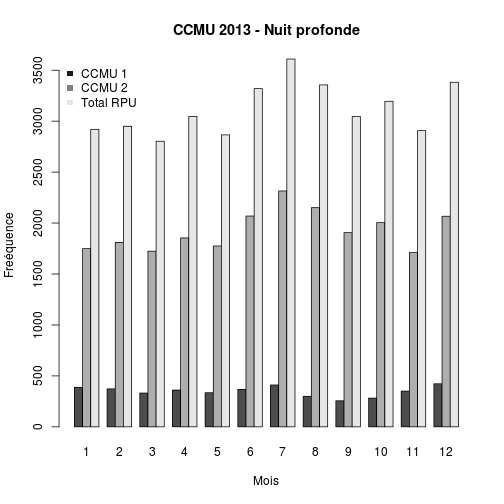
\includegraphics{figure/mois3.png}
\caption{plot of chunk mois}
\end{figure}

\begin{Shaded}
\begin{Highlighting}[]

\CommentTok{# essai de couleurs syntaxe brewer.pal(nb de couleurs,'nom de la palette'))}

\KeywordTok{library}\NormalTok{(RColorBrewer)}
\NormalTok{col =}\StringTok{ }\KeywordTok{brewer.pal}\NormalTok{(}\DecValTok{3}\NormalTok{, }\StringTok{"Set2"}\NormalTok{)}
\KeywordTok{barplot}\NormalTok{(sr, }\DataTypeTok{beside =} \NormalTok{T, }\DataTypeTok{col =} \KeywordTok{brewer.pal}\NormalTok{(}\DecValTok{3}\NormalTok{, }\StringTok{"BuGn"}\NormalTok{))}
\end{Highlighting}
\end{Shaded}

\begin{figure}[htbp]
\centering
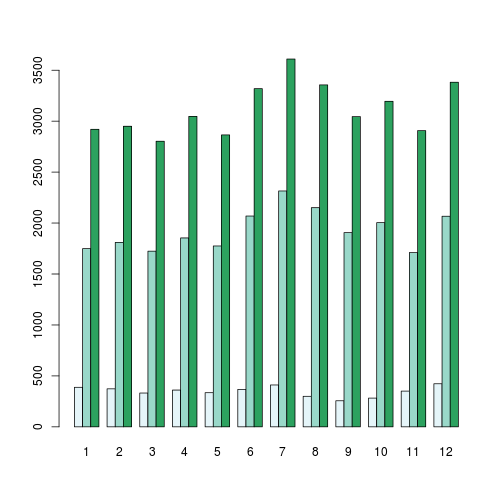
\includegraphics{figure/mois4.png}
\caption{plot of chunk mois}
\end{figure}

\begin{Shaded}
\begin{Highlighting}[]

\KeywordTok{barplot}\NormalTok{(sr, }\DataTypeTok{beside =} \NormalTok{T, }\DataTypeTok{col =} \KeywordTok{brewer.pal}\NormalTok{(}\DecValTok{3}\NormalTok{, }\StringTok{"YlOrRd"}\NormalTok{))}
\end{Highlighting}
\end{Shaded}

\begin{figure}[htbp]
\centering
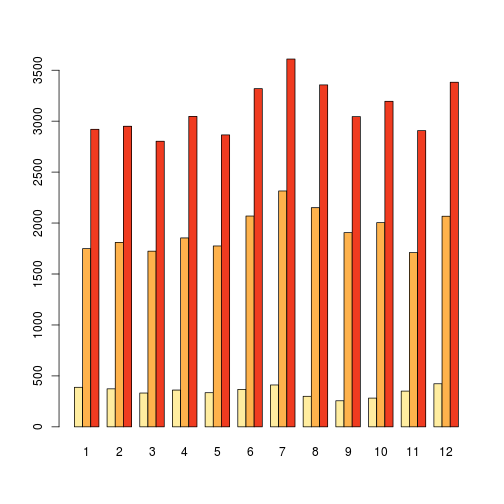
\includegraphics{figure/mois5.png}
\caption{plot of chunk mois}
\end{figure}

\begin{Shaded}
\begin{Highlighting}[]

\KeywordTok{barplot}\NormalTok{(sr, }\DataTypeTok{beside =} \NormalTok{T, }\DataTypeTok{col =} \KeywordTok{brewer.pal}\NormalTok{(}\DecValTok{3}\NormalTok{, }\StringTok{"BuPu"}\NormalTok{))}
\end{Highlighting}
\end{Shaded}

\begin{figure}[htbp]
\centering
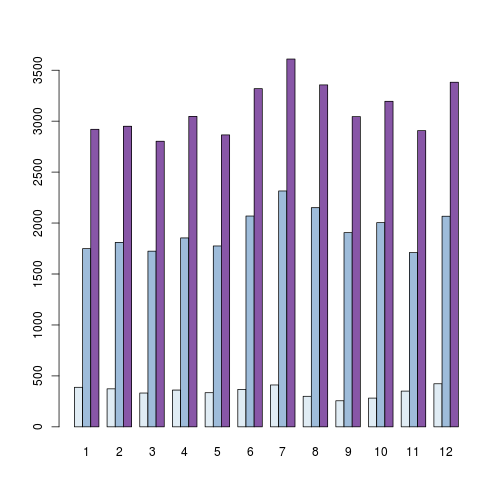
\includegraphics{figure/mois6.png}
\caption{plot of chunk mois}
\end{figure}

\begin{Shaded}
\begin{Highlighting}[]

\KeywordTok{barplot}\NormalTok{(sr, }\DataTypeTok{beside =} \NormalTok{T, }\DataTypeTok{col =} \KeywordTok{brewer.pal}\NormalTok{(}\DecValTok{3}\NormalTok{, }\StringTok{"GnBu"}\NormalTok{))}
\end{Highlighting}
\end{Shaded}

\begin{figure}[htbp]
\centering
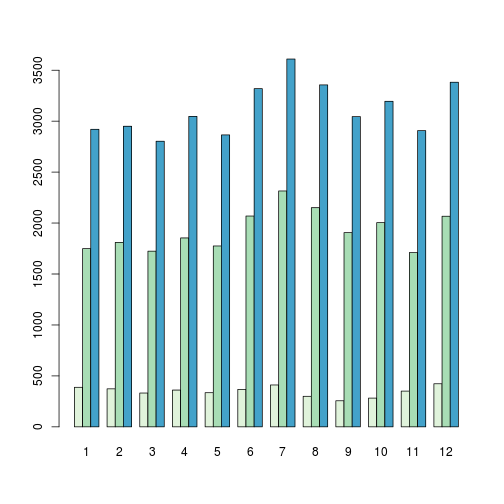
\includegraphics{figure/mois7.png}
\caption{plot of chunk mois}
\end{figure}

\begin{Shaded}
\begin{Highlighting}[]

\KeywordTok{barplot}\NormalTok{(sr, }\DataTypeTok{beside =} \NormalTok{T, }\DataTypeTok{col =} \KeywordTok{brewer.pal}\NormalTok{(}\DecValTok{3}\NormalTok{, }\StringTok{"Greys"}\NormalTok{))}
\end{Highlighting}
\end{Shaded}

\begin{figure}[htbp]
\centering
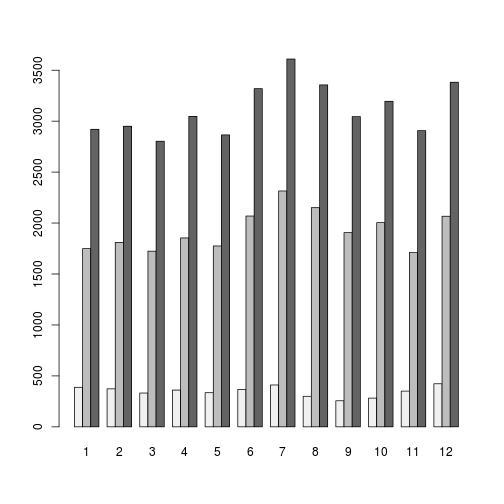
\includegraphics{figure/mois8.png}
\caption{plot of chunk mois}
\end{figure}

\begin{Shaded}
\begin{Highlighting}[]

\KeywordTok{barplot}\NormalTok{(sr, }\DataTypeTok{beside =} \NormalTok{T, }\DataTypeTok{col =} \KeywordTok{brewer.pal}\NormalTok{(}\DecValTok{3}\NormalTok{, }\StringTok{"Oranges"}\NormalTok{))}
\end{Highlighting}
\end{Shaded}

\begin{figure}[htbp]
\centering
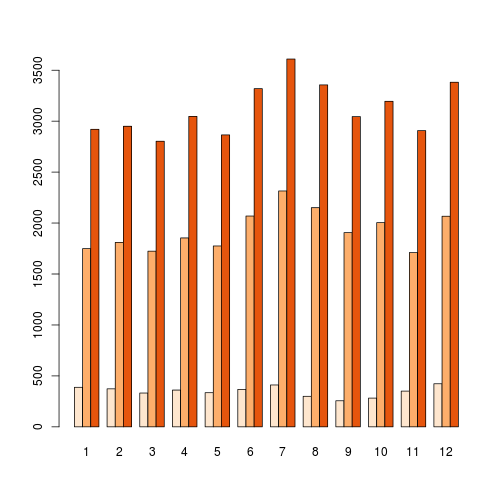
\includegraphics{figure/mois9.png}
\caption{plot of chunk mois}
\end{figure}

\begin{Shaded}
\begin{Highlighting}[]

\KeywordTok{barplot}\NormalTok{(sr, }\DataTypeTok{beside =} \NormalTok{T, }\DataTypeTok{col =} \KeywordTok{brewer.pal}\NormalTok{(}\DecValTok{3}\NormalTok{, }\StringTok{"Purples"}\NormalTok{))}
\end{Highlighting}
\end{Shaded}

\begin{figure}[htbp]
\centering
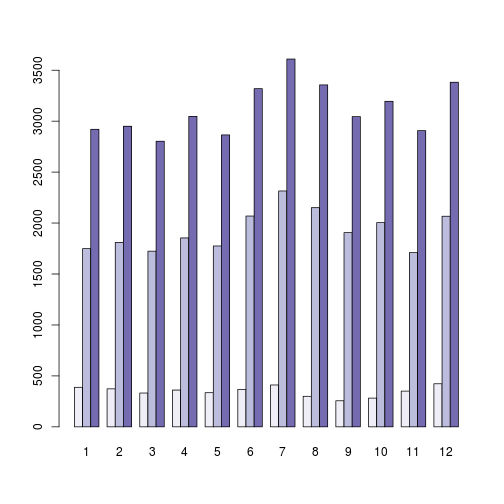
\includegraphics{figure/mois10.png}
\caption{plot of chunk mois}
\end{figure}

\begin{Shaded}
\begin{Highlighting}[]

\NormalTok{col =}\StringTok{ }\KeywordTok{brewer.pal}\NormalTok{(}\DecValTok{3}\NormalTok{, }\StringTok{"Blues"}\NormalTok{)}
\KeywordTok{barplot}\NormalTok{(sr, }\DataTypeTok{beside =} \NormalTok{T, }\DataTypeTok{ylab =} \StringTok{"Freéquence"}\NormalTok{, }\DataTypeTok{xlab =} \StringTok{"Mois"}\NormalTok{, }\DataTypeTok{main =} \StringTok{"CCMU 2013 - Nuit profonde"}\NormalTok{, }
    \DataTypeTok{col =} \NormalTok{col)}
\KeywordTok{legend}\NormalTok{(}\StringTok{"topleft"}\NormalTok{, }\DataTypeTok{legend =} \KeywordTok{c}\NormalTok{(}\StringTok{"CCMU 1"}\NormalTok{, }\StringTok{"CCMU 2"}\NormalTok{, }\StringTok{"Total RPU"}\NormalTok{), }\DataTypeTok{col =} \NormalTok{col, }\DataTypeTok{pch =} \DecValTok{15}\NormalTok{, }
    \DataTypeTok{bty =} \StringTok{"n"}\NormalTok{)}
\end{Highlighting}
\end{Shaded}

\begin{figure}[htbp]
\centering
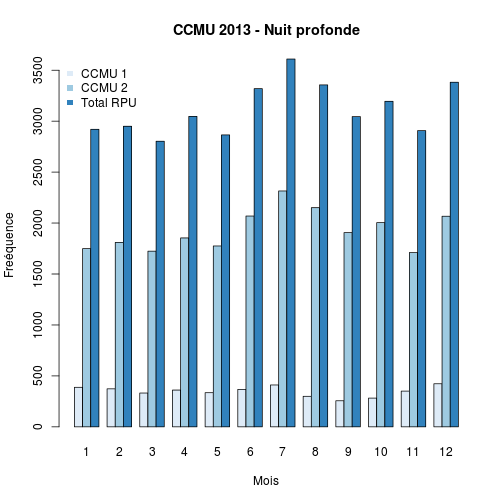
\includegraphics{figure/mois11.png}
\caption{plot of chunk mois}
\end{figure}

\begin{Shaded}
\begin{Highlighting}[]

\CommentTok{# CCMU1 soirée et nuit profonde ==============================}

\NormalTok{YL <-}\StringTok{ }\KeywordTok{c}\NormalTok{(}\KeywordTok{min}\NormalTok{(}\KeywordTok{min}\NormalTok{(t_dnp1), }\KeywordTok{min}\NormalTok{(t_dsr1)), }\KeywordTok{max}\NormalTok{(}\KeywordTok{max}\NormalTok{(t_dnp1), }\KeywordTok{max}\NormalTok{(t_dsr1)))}
\KeywordTok{plot}\NormalTok{(t_dsr1, }\DataTypeTok{type =} \StringTok{"l"}\NormalTok{, }\DataTypeTok{ylim =} \NormalTok{YL, }\DataTypeTok{col =} \StringTok{"green"}\NormalTok{, }\DataTypeTok{ylab =} \StringTok{"Fréquence"}\NormalTok{, }\DataTypeTok{xlab =} \StringTok{"Mois"}\NormalTok{, }
    \DataTypeTok{main =} \StringTok{"CCMU1 2013 (avant et après minuit)"}\NormalTok{)}
\KeywordTok{lines}\NormalTok{(t_dnp1, }\DataTypeTok{col =} \StringTok{"blue"}\NormalTok{, }\DataTypeTok{ylim =} \NormalTok{YL)}
\KeywordTok{abline}\NormalTok{(}\DataTypeTok{h =} \KeywordTok{mean}\NormalTok{(t_dsr1), }\DataTypeTok{lty =} \DecValTok{2}\NormalTok{, }\DataTypeTok{col =} \StringTok{"green"}\NormalTok{)}
\KeywordTok{abline}\NormalTok{(}\DataTypeTok{h =} \KeywordTok{mean}\NormalTok{(t_dnp1), }\DataTypeTok{lty =} \DecValTok{2}\NormalTok{, }\DataTypeTok{col =} \StringTok{"blue"}\NormalTok{)}
\KeywordTok{text}\NormalTok{(}\DecValTok{10}\NormalTok{, }\KeywordTok{mean}\NormalTok{(t_dsr1) +}\StringTok{ }\DecValTok{10}\NormalTok{, }\KeywordTok{paste}\NormalTok{(}\StringTok{"moyenne"}\NormalTok{, }\KeywordTok{round}\NormalTok{(}\KeywordTok{mean}\NormalTok{(t_dsr1), }\DecValTok{2}\NormalTok{)), }\DataTypeTok{col =} \StringTok{"green"}\NormalTok{)}
\KeywordTok{text}\NormalTok{(}\DecValTok{10}\NormalTok{, }\KeywordTok{mean}\NormalTok{(t_dnp1) +}\StringTok{ }\DecValTok{10}\NormalTok{, }\KeywordTok{paste}\NormalTok{(}\StringTok{"moyenne"}\NormalTok{, }\KeywordTok{round}\NormalTok{(}\KeywordTok{mean}\NormalTok{(t_dnp1), }\DecValTok{2}\NormalTok{)), }\DataTypeTok{col =} \StringTok{"blue"}\NormalTok{)}
\KeywordTok{legend}\NormalTok{(}\StringTok{"topleft"}\NormalTok{, }\DataTypeTok{legend =} \KeywordTok{c}\NormalTok{(}\StringTok{"soirée"}\NormalTok{, }\StringTok{"nuit profonde"}\NormalTok{), }\DataTypeTok{col =} \KeywordTok{c}\NormalTok{(}\StringTok{"green"}\NormalTok{, }\StringTok{"blue"}\NormalTok{), }
    \DataTypeTok{lty =} \DecValTok{1}\NormalTok{)}
\end{Highlighting}
\end{Shaded}

\begin{figure}[htbp]
\centering
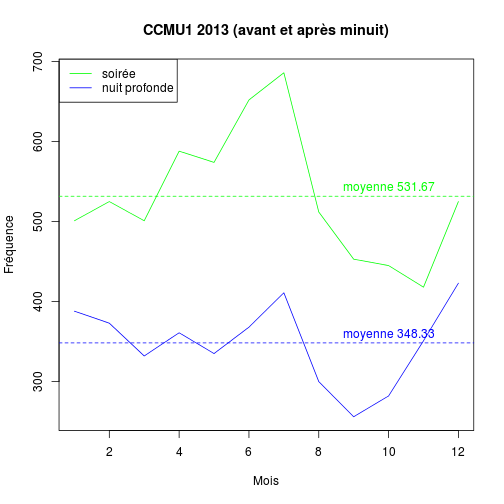
\includegraphics{figure/mois12.png}
\caption{plot of chunk mois}
\end{figure}

\begin{Shaded}
\begin{Highlighting}[]

\CommentTok{# CCMU2 soirée et nuit profonde ==============================}

\NormalTok{YL <-}\StringTok{ }\KeywordTok{c}\NormalTok{(}\KeywordTok{min}\NormalTok{(}\KeywordTok{min}\NormalTok{(t_dnp2), }\KeywordTok{min}\NormalTok{(t_dsr2)), }\KeywordTok{max}\NormalTok{(}\KeywordTok{max}\NormalTok{(t_dnp2), }\KeywordTok{max}\NormalTok{(t_dsr2)))}
\KeywordTok{plot}\NormalTok{(t_dsr2, }\DataTypeTok{type =} \StringTok{"l"}\NormalTok{, }\DataTypeTok{ylim =} \NormalTok{YL, }\DataTypeTok{col =} \StringTok{"green"}\NormalTok{, }\DataTypeTok{ylab =} \StringTok{"Fréquence"}\NormalTok{, }\DataTypeTok{xlab =} \StringTok{"Mois"}\NormalTok{, }
    \DataTypeTok{main =} \StringTok{"CCMU2 2013 (avant et après minuit)"}\NormalTok{)}
\KeywordTok{lines}\NormalTok{(t_dnp2, }\DataTypeTok{col =} \StringTok{"blue"}\NormalTok{, }\DataTypeTok{ylim =} \NormalTok{YL)}

\KeywordTok{abline}\NormalTok{(}\DataTypeTok{h =} \KeywordTok{mean}\NormalTok{(t_dsr2), }\DataTypeTok{lty =} \DecValTok{2}\NormalTok{, }\DataTypeTok{col =} \StringTok{"green"}\NormalTok{)}
\KeywordTok{abline}\NormalTok{(}\DataTypeTok{h =} \KeywordTok{mean}\NormalTok{(t_dnp2), }\DataTypeTok{lty =} \DecValTok{2}\NormalTok{, }\DataTypeTok{col =} \StringTok{"blue"}\NormalTok{)}

\KeywordTok{text}\NormalTok{(}\DecValTok{10}\NormalTok{, }\KeywordTok{mean}\NormalTok{(t_dsr2) +}\StringTok{ }\DecValTok{10}\NormalTok{, }\KeywordTok{paste}\NormalTok{(}\StringTok{"moyenne"}\NormalTok{, }\KeywordTok{round}\NormalTok{(}\KeywordTok{mean}\NormalTok{(t_dsr2), }\DecValTok{2}\NormalTok{)), }\DataTypeTok{col =} \StringTok{"green"}\NormalTok{)}
\KeywordTok{text}\NormalTok{(}\DecValTok{10}\NormalTok{, }\KeywordTok{mean}\NormalTok{(t_dnp2) +}\StringTok{ }\DecValTok{10}\NormalTok{, }\KeywordTok{paste}\NormalTok{(}\StringTok{"moyenne"}\NormalTok{, }\KeywordTok{round}\NormalTok{(}\KeywordTok{mean}\NormalTok{(t_dnp2), }\DecValTok{2}\NormalTok{)), }\DataTypeTok{col =} \StringTok{"blue"}\NormalTok{)}
\KeywordTok{legend}\NormalTok{(}\StringTok{"topleft"}\NormalTok{, }\DataTypeTok{legend =} \KeywordTok{c}\NormalTok{(}\StringTok{"soirée"}\NormalTok{, }\StringTok{"nuit profonde"}\NormalTok{), }\DataTypeTok{col =} \KeywordTok{c}\NormalTok{(}\StringTok{"green"}\NormalTok{, }\StringTok{"blue"}\NormalTok{), }
    \DataTypeTok{lty =} \DecValTok{1}\NormalTok{)}
\end{Highlighting}
\end{Shaded}

\begin{figure}[htbp]
\centering
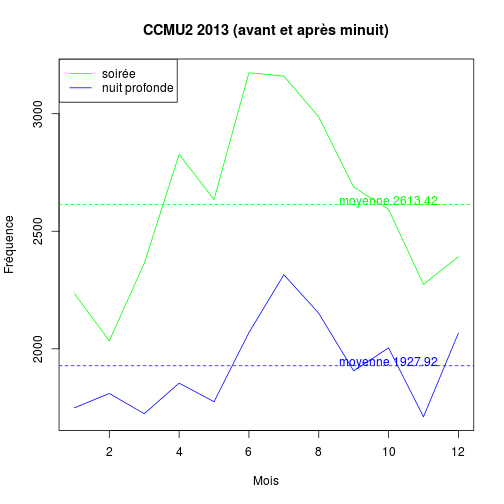
\includegraphics{figure/mois13.png}
\caption{plot of chunk mois}
\end{figure}

\subsection{Comparaison passages totaux versus CCMU1 et 2}

\begin{Shaded}
\begin{Highlighting}[]
\NormalTok{YL <-}\StringTok{ }\KeywordTok{c}\NormalTok{(}\KeywordTok{min}\NormalTok{(t_dsr1), }\KeywordTok{max}\NormalTok{(t_dsrt))}
\KeywordTok{plot}\NormalTok{(t_dsr1, }\DataTypeTok{type =} \StringTok{"l"}\NormalTok{, }\DataTypeTok{col =} \StringTok{"green"}\NormalTok{, }\DataTypeTok{ylim =} \NormalTok{YL, }\DataTypeTok{xlab =} \StringTok{"Mois"}\NormalTok{, }\DataTypeTok{ylab =} \StringTok{"RPU"}\NormalTok{, }
    \DataTypeTok{main =} \StringTok{"Comparaison passages totaux ~ CCMU 1 & 2 en soirée"}\NormalTok{)}
\KeywordTok{lines}\NormalTok{(t_dsrt, }\DataTypeTok{ylim =} \NormalTok{YL, }\DataTypeTok{col =} \StringTok{"red"}\NormalTok{)}
\KeywordTok{lines}\NormalTok{(t_dsr2, }\DataTypeTok{ylim =} \NormalTok{YL, }\DataTypeTok{col =} \StringTok{"blue"}\NormalTok{)}
\KeywordTok{legend}\NormalTok{(}\StringTok{"topleft"}\NormalTok{, }\DataTypeTok{legend =} \KeywordTok{c}\NormalTok{(}\StringTok{"total"}\NormalTok{, }\StringTok{"CCMU 1"}\NormalTok{, }\StringTok{"CCMU 2"}\NormalTok{), }\DataTypeTok{col =} \KeywordTok{c}\NormalTok{(}\StringTok{"red"}\NormalTok{, }\StringTok{"green"}\NormalTok{, }
    \StringTok{"blue"}\NormalTok{), }\DataTypeTok{lty =} \DecValTok{1}\NormalTok{, }\DataTypeTok{bty =} \StringTok{"n"}\NormalTok{)}
\end{Highlighting}
\end{Shaded}

\begin{figure}[htbp]
\centering
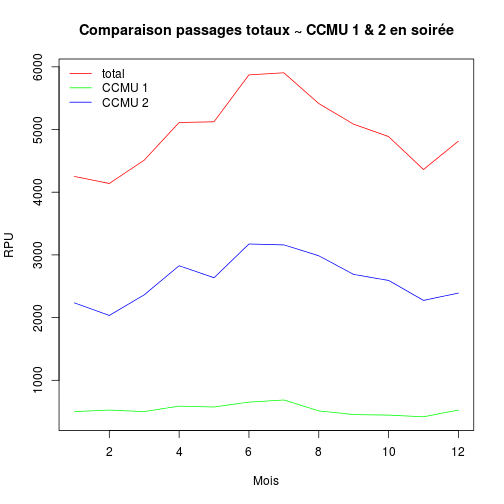
\includegraphics{figure/soiree_tot_ccmu1.png}
\caption{plot of chunk soiree\_tot\_ccmu}
\end{figure}

\begin{Shaded}
\begin{Highlighting}[]

\NormalTok{YL <-}\StringTok{ }\KeywordTok{c}\NormalTok{(}\KeywordTok{min}\NormalTok{(t_dnp1), }\KeywordTok{max}\NormalTok{(t_dnpt))}
\KeywordTok{plot}\NormalTok{(t_dnp1, }\DataTypeTok{type =} \StringTok{"l"}\NormalTok{, }\DataTypeTok{col =} \StringTok{"green"}\NormalTok{, }\DataTypeTok{ylim =} \NormalTok{YL, }\DataTypeTok{xlab =} \StringTok{"Mois"}\NormalTok{, }\DataTypeTok{ylab =} \StringTok{"RPU"}\NormalTok{, }
    \DataTypeTok{main =} \StringTok{"Comparaison passages totaux ~ CCMU 1 & 2 en Nuit profonde"}\NormalTok{)}
\KeywordTok{lines}\NormalTok{(t_dnpt, }\DataTypeTok{ylim =} \NormalTok{YL, }\DataTypeTok{col =} \StringTok{"red"}\NormalTok{)}
\KeywordTok{lines}\NormalTok{(t_dnp2, }\DataTypeTok{ylim =} \NormalTok{YL, }\DataTypeTok{col =} \StringTok{"blue"}\NormalTok{)}
\KeywordTok{legend}\NormalTok{(}\StringTok{"topleft"}\NormalTok{, }\DataTypeTok{legend =} \KeywordTok{c}\NormalTok{(}\StringTok{"total"}\NormalTok{, }\StringTok{"CCMU 1"}\NormalTok{, }\StringTok{"CCMU 2"}\NormalTok{), }\DataTypeTok{col =} \KeywordTok{c}\NormalTok{(}\StringTok{"red"}\NormalTok{, }\StringTok{"green"}\NormalTok{, }
    \StringTok{"blue"}\NormalTok{), }\DataTypeTok{lty =} \DecValTok{1}\NormalTok{, }\DataTypeTok{bty =} \StringTok{"n"}\NormalTok{)}
\end{Highlighting}
\end{Shaded}

\begin{figure}[htbp]
\centering
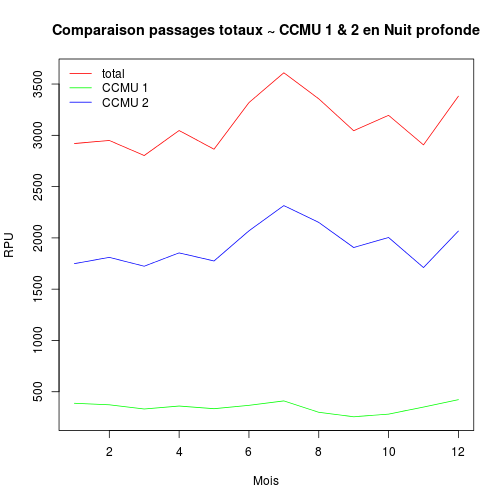
\includegraphics{figure/soiree_tot_ccmu2.png}
\caption{plot of chunk soiree\_tot\_ccmu}
\end{figure}
